
\setlength{\parskip}{0pt} % Espaciado compacto
\setlength{\parindent}{0em}

% Configuración del entorno "Solución"
\theoremstyle{nonumberplain}
\theoremheaderfont{\itshape}
\theorembodyfont{\upshape}
\theoremseparator{.}
\theoremsymbol{\ensuremath{\square}}
\newtheorem{solucion}{Solución}

\begin{document}

\textbf{Problema:} Encuentre la mejor aproximación cuadrática de la función \( f(x, y) = (x+1)e^y \) en una vecindad del punto \( (0, 0) \). \\

\begin{solucion}
La aproximación cuadrática de Taylor para una función de dos variables \( f(x, y) \) alrededor del punto \( (a, b) \) está dada por:
\[
P_2(x, y) = f(a, b) + f_x(a, b)(x - a) + f_y(a, b)(y - b) + \frac{1}{2} \left[ f_{xx}(a, b)(x - a)^2 + 2f_{xy}(a, b)(x - a)(y - b) + f_{yy}(a, b)(y - b)^2 \right]
\]
En este caso, \( a = 0 \) y \( b = 0 \), por lo que:
\[
P_2(x, y) = f(0, 0) + f_x(0, 0)x + f_y(0, 0)y + \frac{1}{2} \left[ f_{xx}(0, 0)x^2 + 2f_{xy}(0, 0)xy + f_{yy}(0, 0)y^2 \right]
\]
**Cálculo de derivadas:**
\[
f(0, 0) = 1, \quad f_x(x, y) = e^y \implies f_x(0, 0) = 1, \quad f_y(x, y) = (x+1)e^y \implies f_y(0, 0) = 1
\]
\[
f_{xx}(x, y) = 0, \quad f_{yy}(x, y) = (x+1)e^y \implies f_{yy}(0, 0) = 1, \quad f_{xy}(x, y) = e^y \implies f_{xy}(0, 0) = 1
\]
Sustituyendo:
\[
P_2(x, y) = 1 + x + y + \frac{1}{2} \left[ 0 \cdot x^2 + 2 \cdot 1 \cdot xy + 1 \cdot y^2 \right]
\]
Simplificando:
\[
P_2(x, y) = 1 + x + y + xy + \frac{1}{2}y^2
\]
Por lo tanto, la mejor aproximación cuadrática es:
\[
P_2(x, y) = 1 + x + y + xy + \frac{1}{2}y^2
\]

\begin{figure}[h]
    \centering
    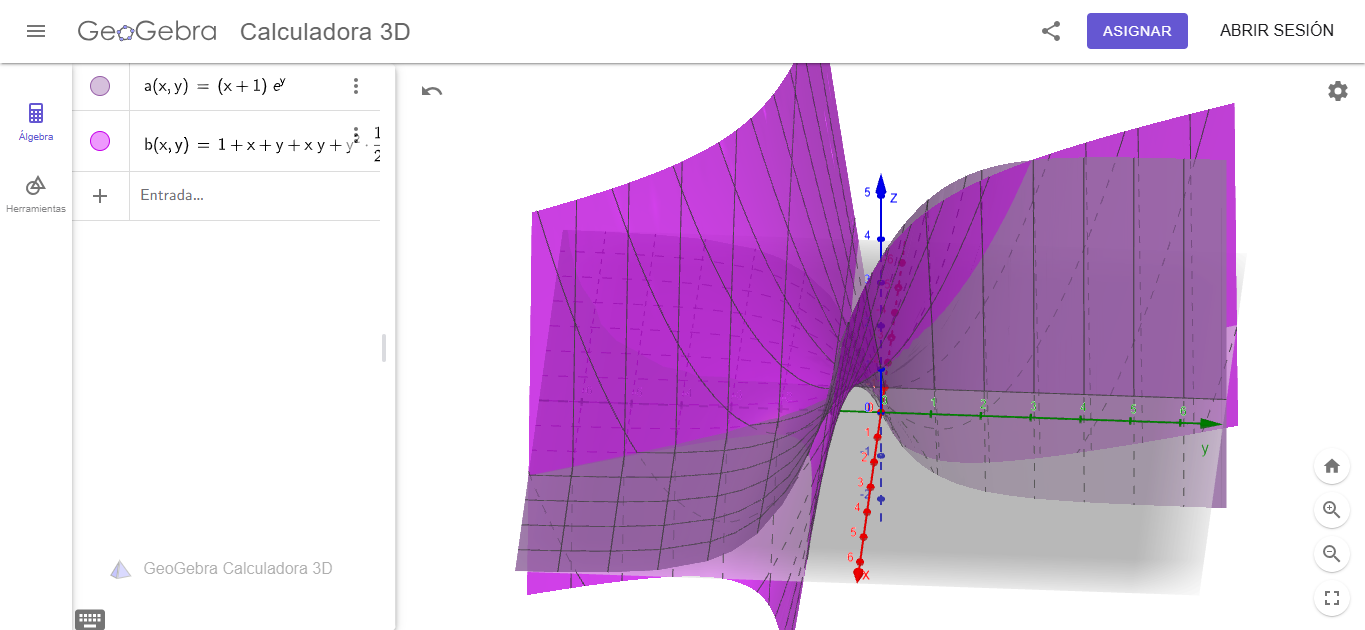
\includegraphics[width=0.75\linewidth]{imagen.png}
    \caption{Comparación de la función con su aproximación cuadrática.}
\end{figure}

\end{solucion}

\end{document}
